% !TEX root = ../main.tex
\begin{figure}[t]
\label{fig:bptt}
\iflatexml
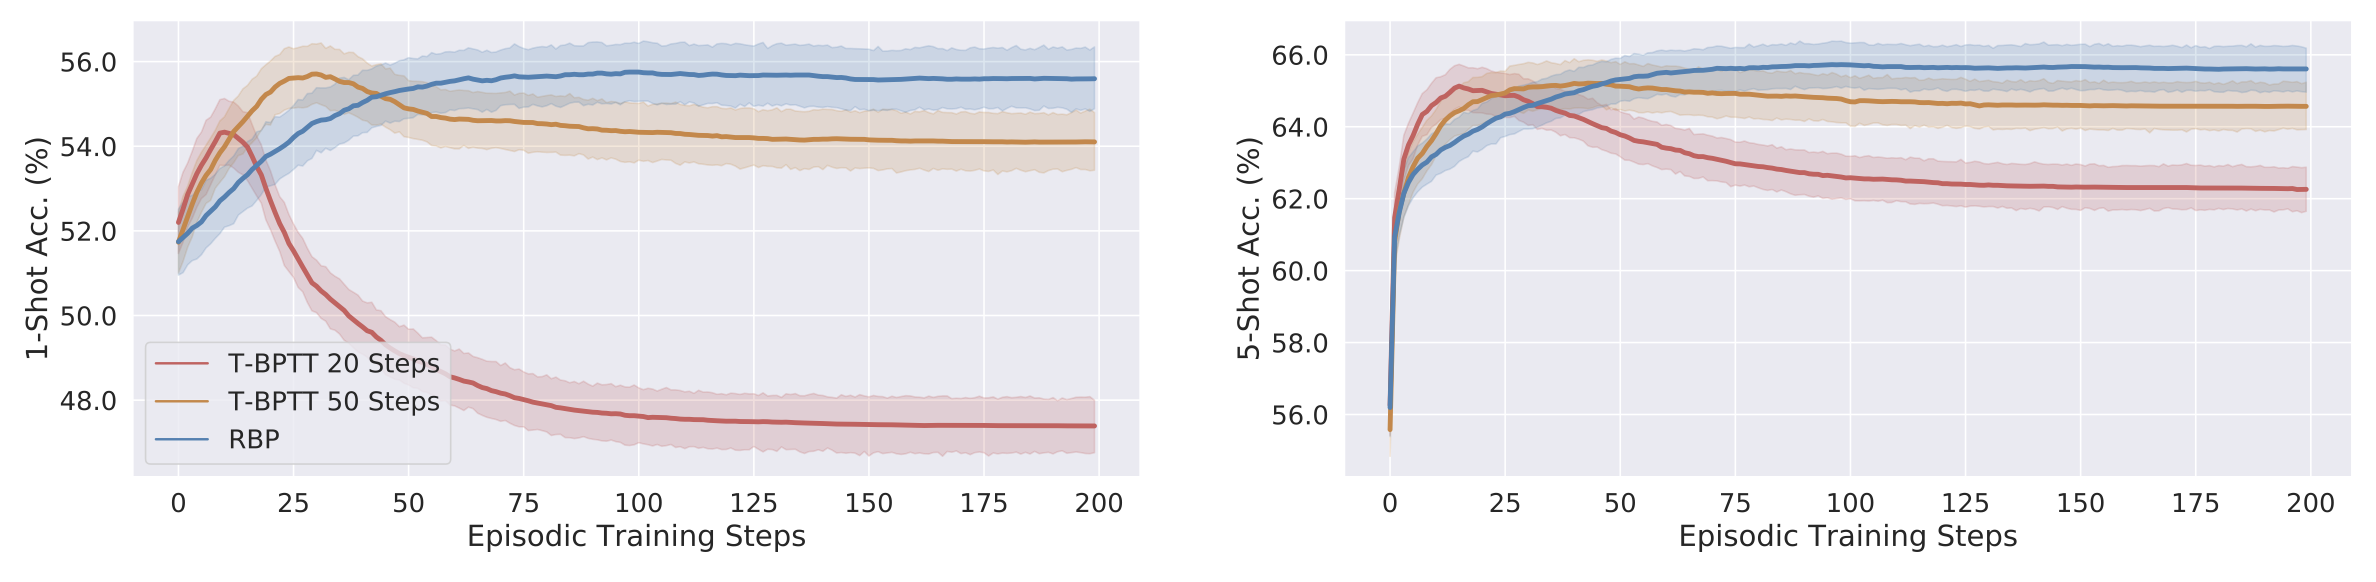
\includegraphics[width=6\textwidth]{figures/bptt.png}
\else
\begin{minipage}[c]{\textwidth}
\centering
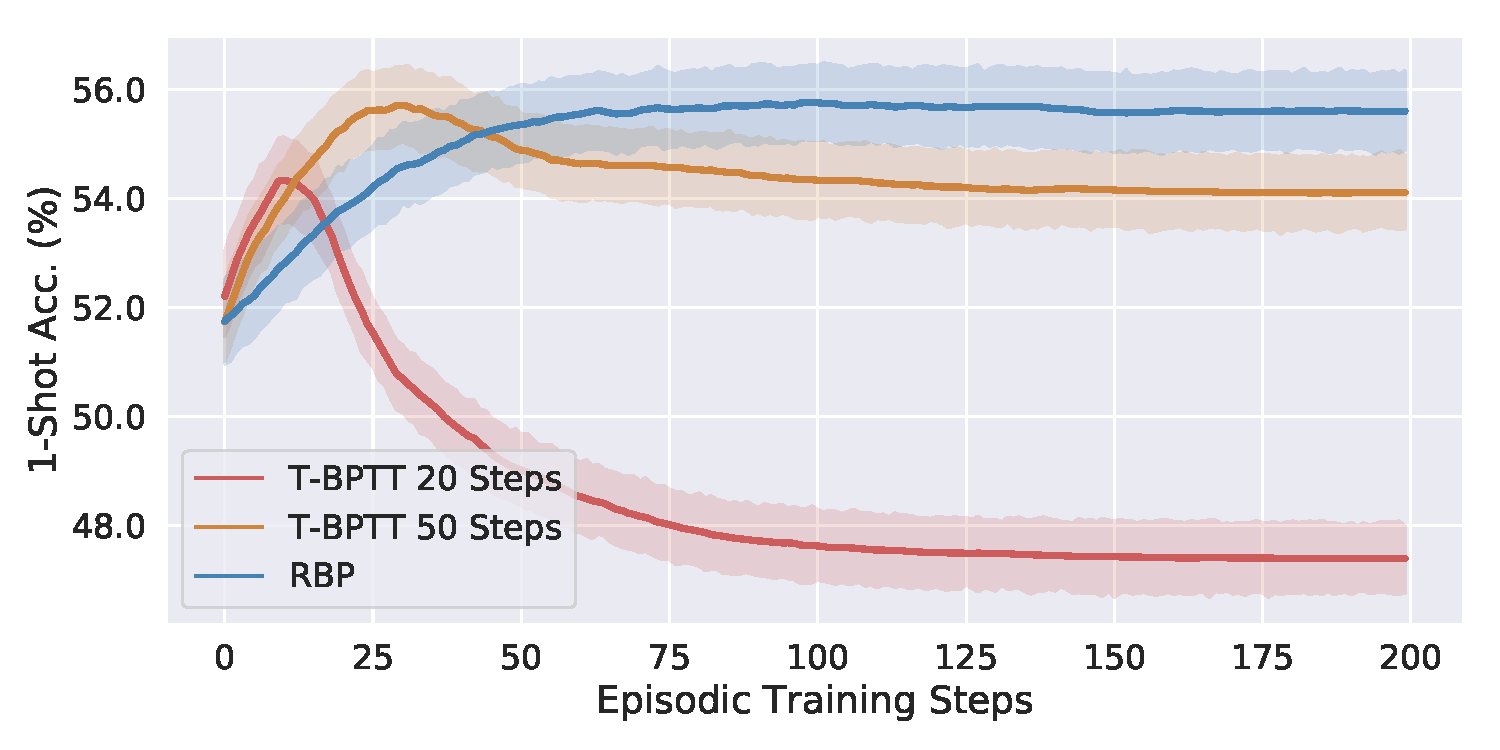
\includegraphics[width=0.49\textwidth,trim={0cm 0cm 0cm 0cm},clip]{figures/example.pdf}
\hfill
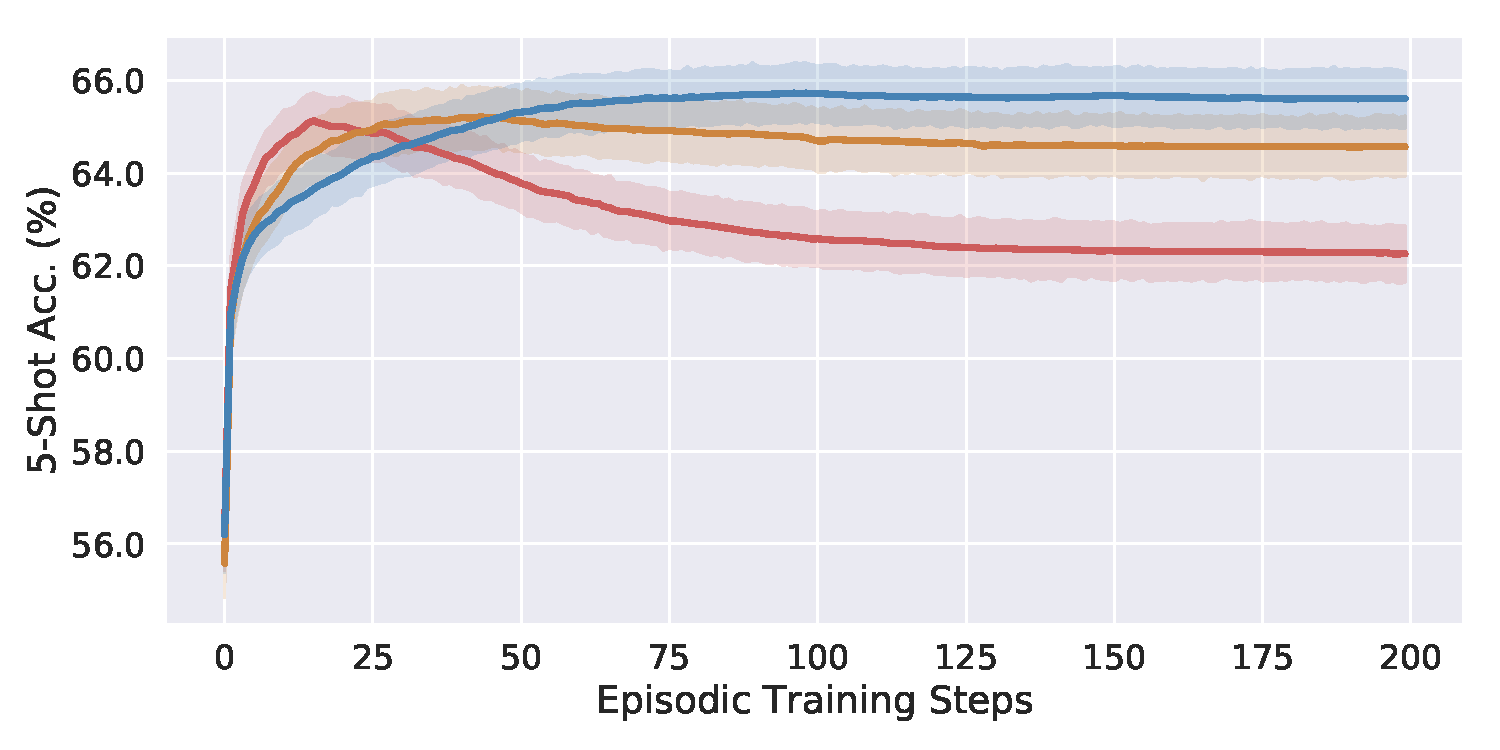
\includegraphics[width=0.49\textwidth,trim={0cm 0cm 0cm 0cm},clip]{figures/example-s5.pdf}
\end{minipage}
\fi
\caption{Learning the proposed model using truncated BPTT vs. RBP. Models
are evaluated with 1-shot (left) and 5-shot (right) 64+5-way episodes,
with various number of gradient descent steps.}
\label{fig:bptt}
\end{figure}